\begin{center}
    PRACTICA DE LABORATORIO N° 01
\end{center}

\section{OBJETIVOS}
Elaboración de Dashboards en Power BI

\section{REQUERIMIENTOS}

\begin{itemize}

- Conocimientos básicos de administración de base de datos Microsoft   SQL Server.
\\- Conocimientos básicos de SQL.
\\- Microsoft SQL Server 2016 o superior
\\- Base de datos AdventureWorks2016 o superior
\\- Power BI Desktop.
\\- Tener una cuenta Microsoft registrada en el Portal de Power Bi.
\end{itemize}

\section{DESARROLLO} 

\begin{itemize}
1. Iniciar Power BI Desktop.
\end{itemize} 

\begin{center}
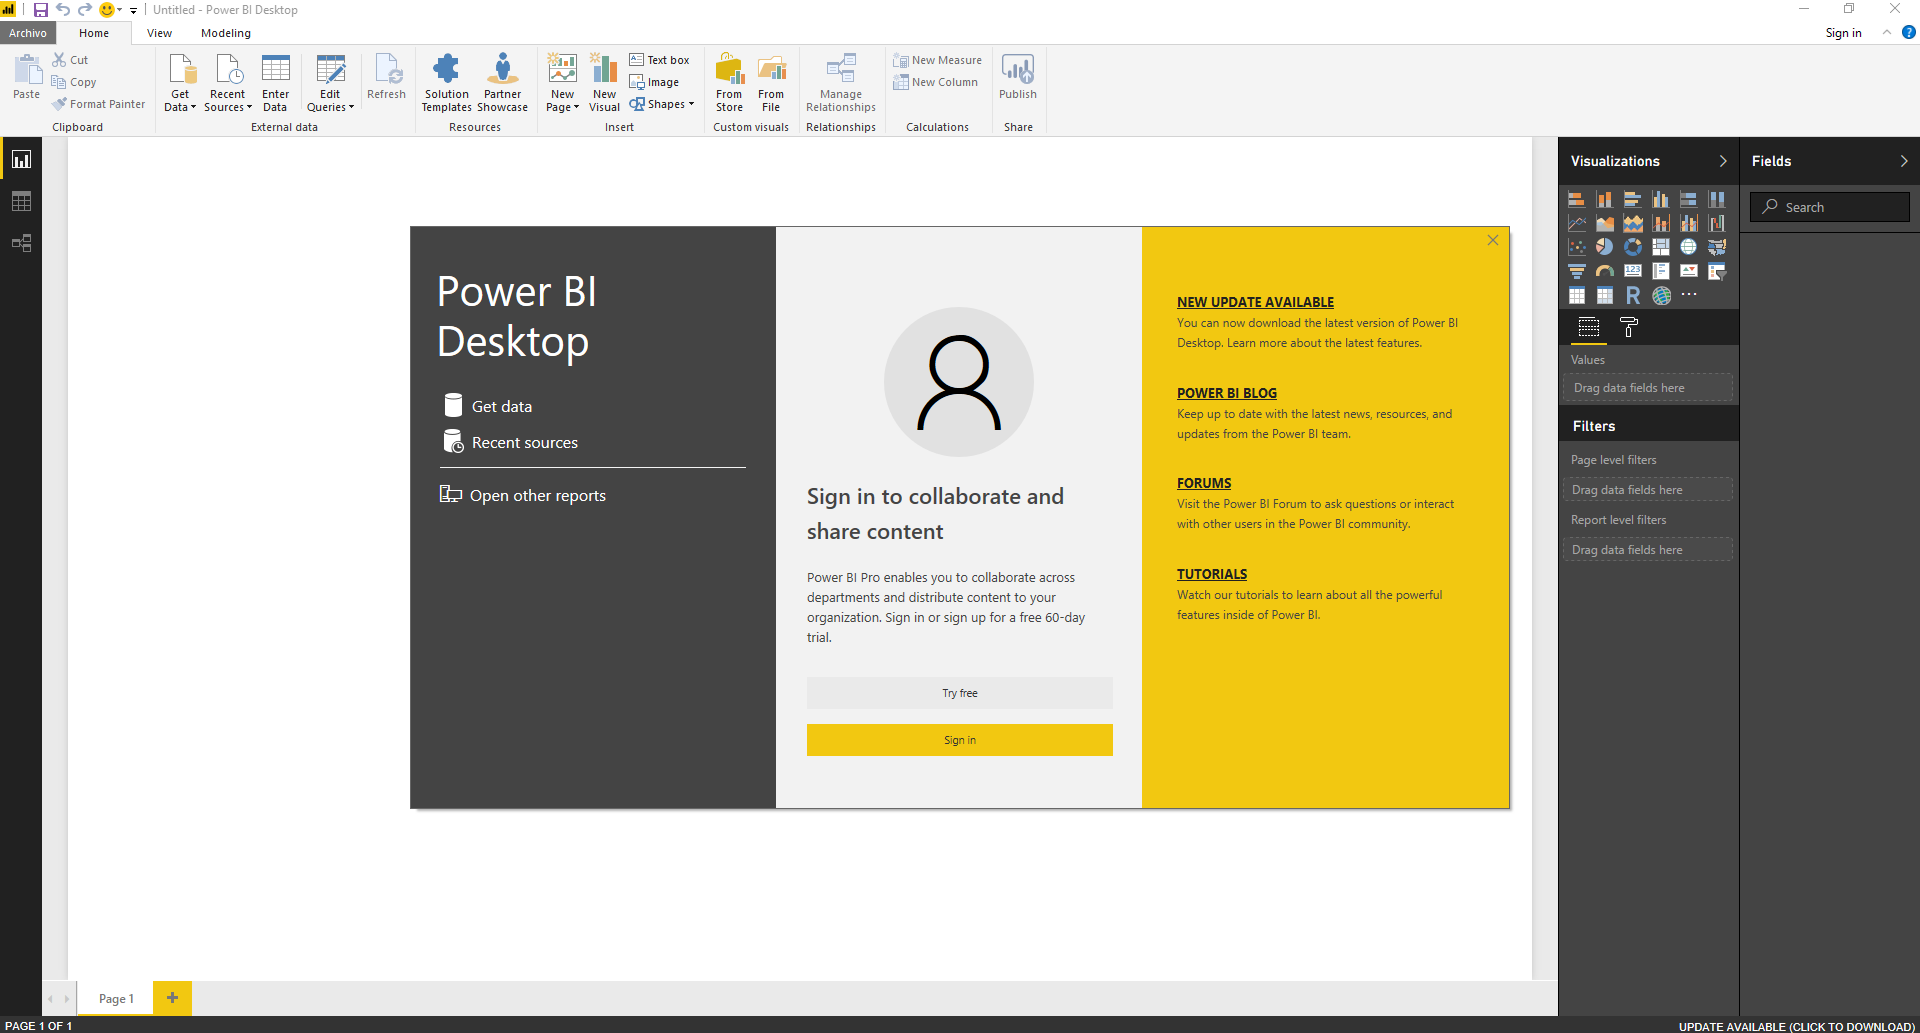
\includegraphics[width=15cm]{./Imagenes/imagen1} 
\end{center}

\begin{itemize}
2. Conectar a SQL Server desde Power BI Desktop 
\end{itemize} 

\begin{center}
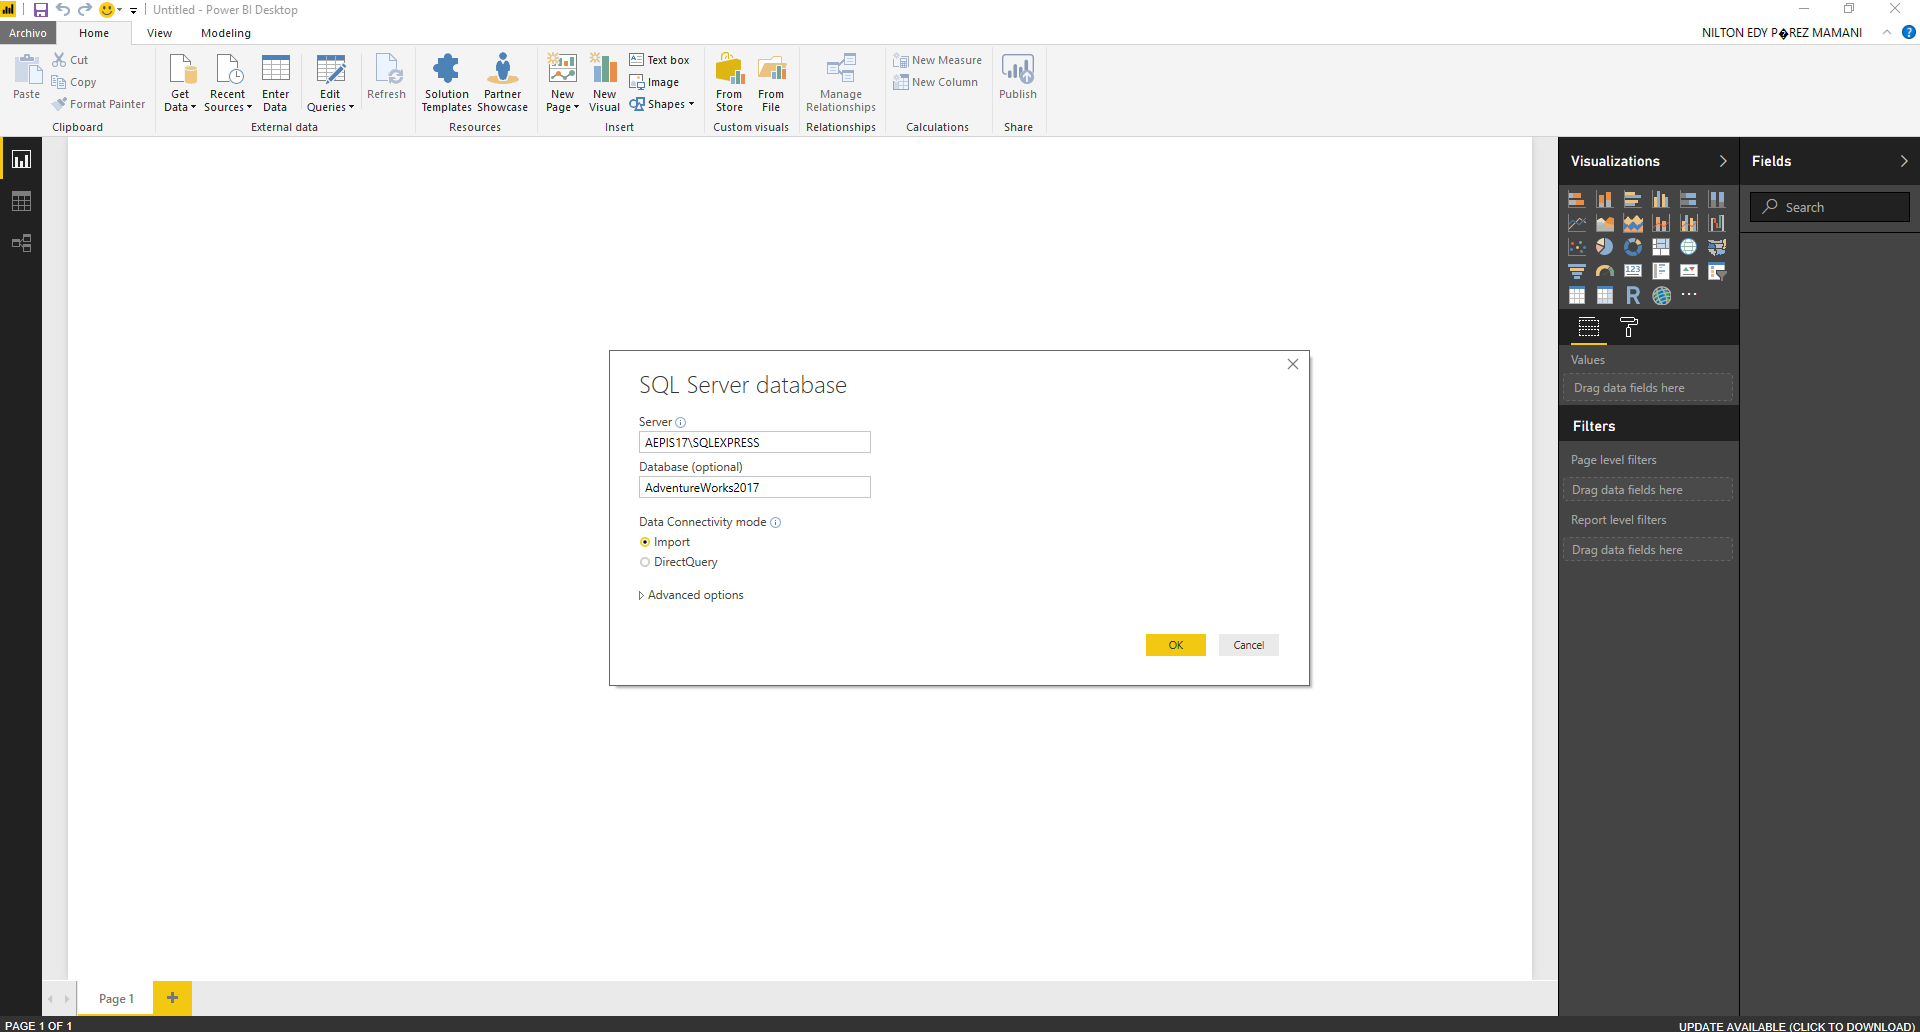
\includegraphics[width=15cm]{./Imagenes/imagen2} 
\end{center}

\begin{itemize}
3. Generar un reporte que muestre a todo el personal de ventas 
\end{itemize} 

\begin{center}
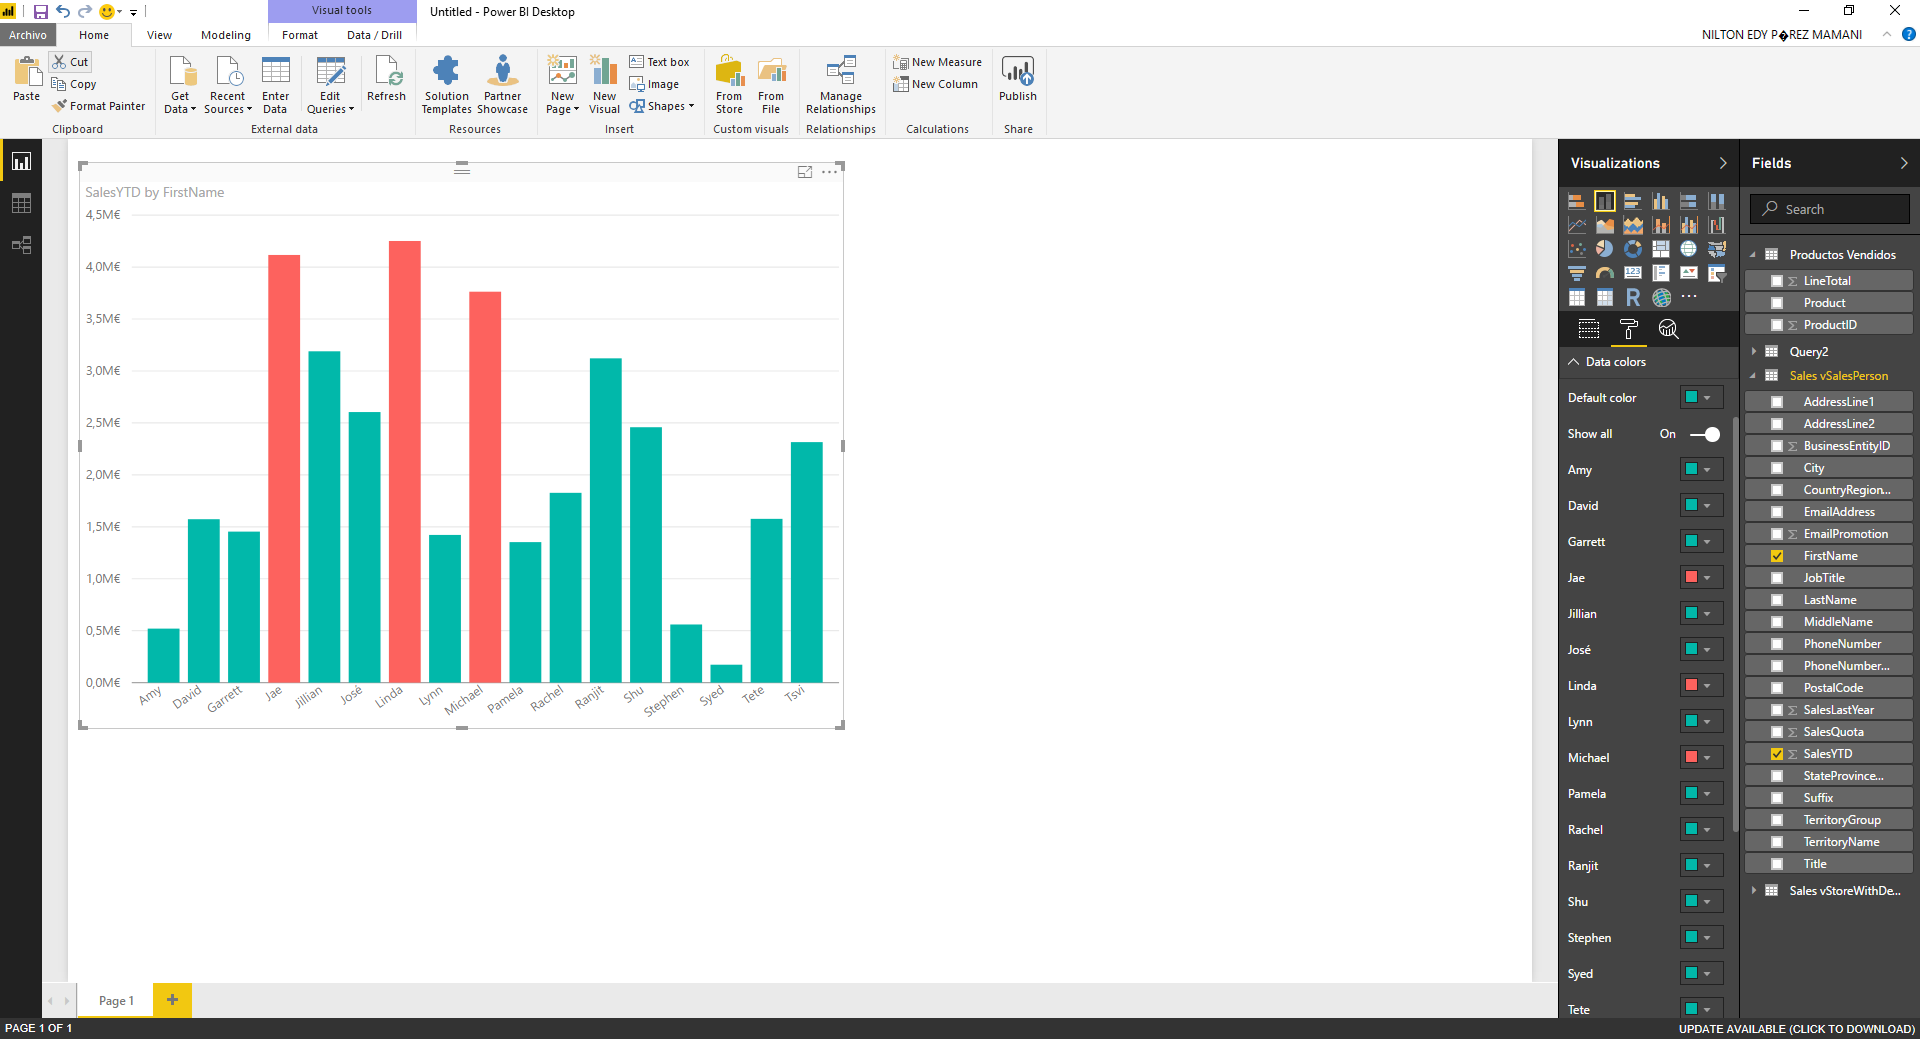
\includegraphics[width=15cm]{./Imagenes/imagen3} 
\end{center}

\begin{itemize}
4. Generar un area de reporte que muestre todo los resultados que indica el trabajo
\end{itemize} 

\begin{center}
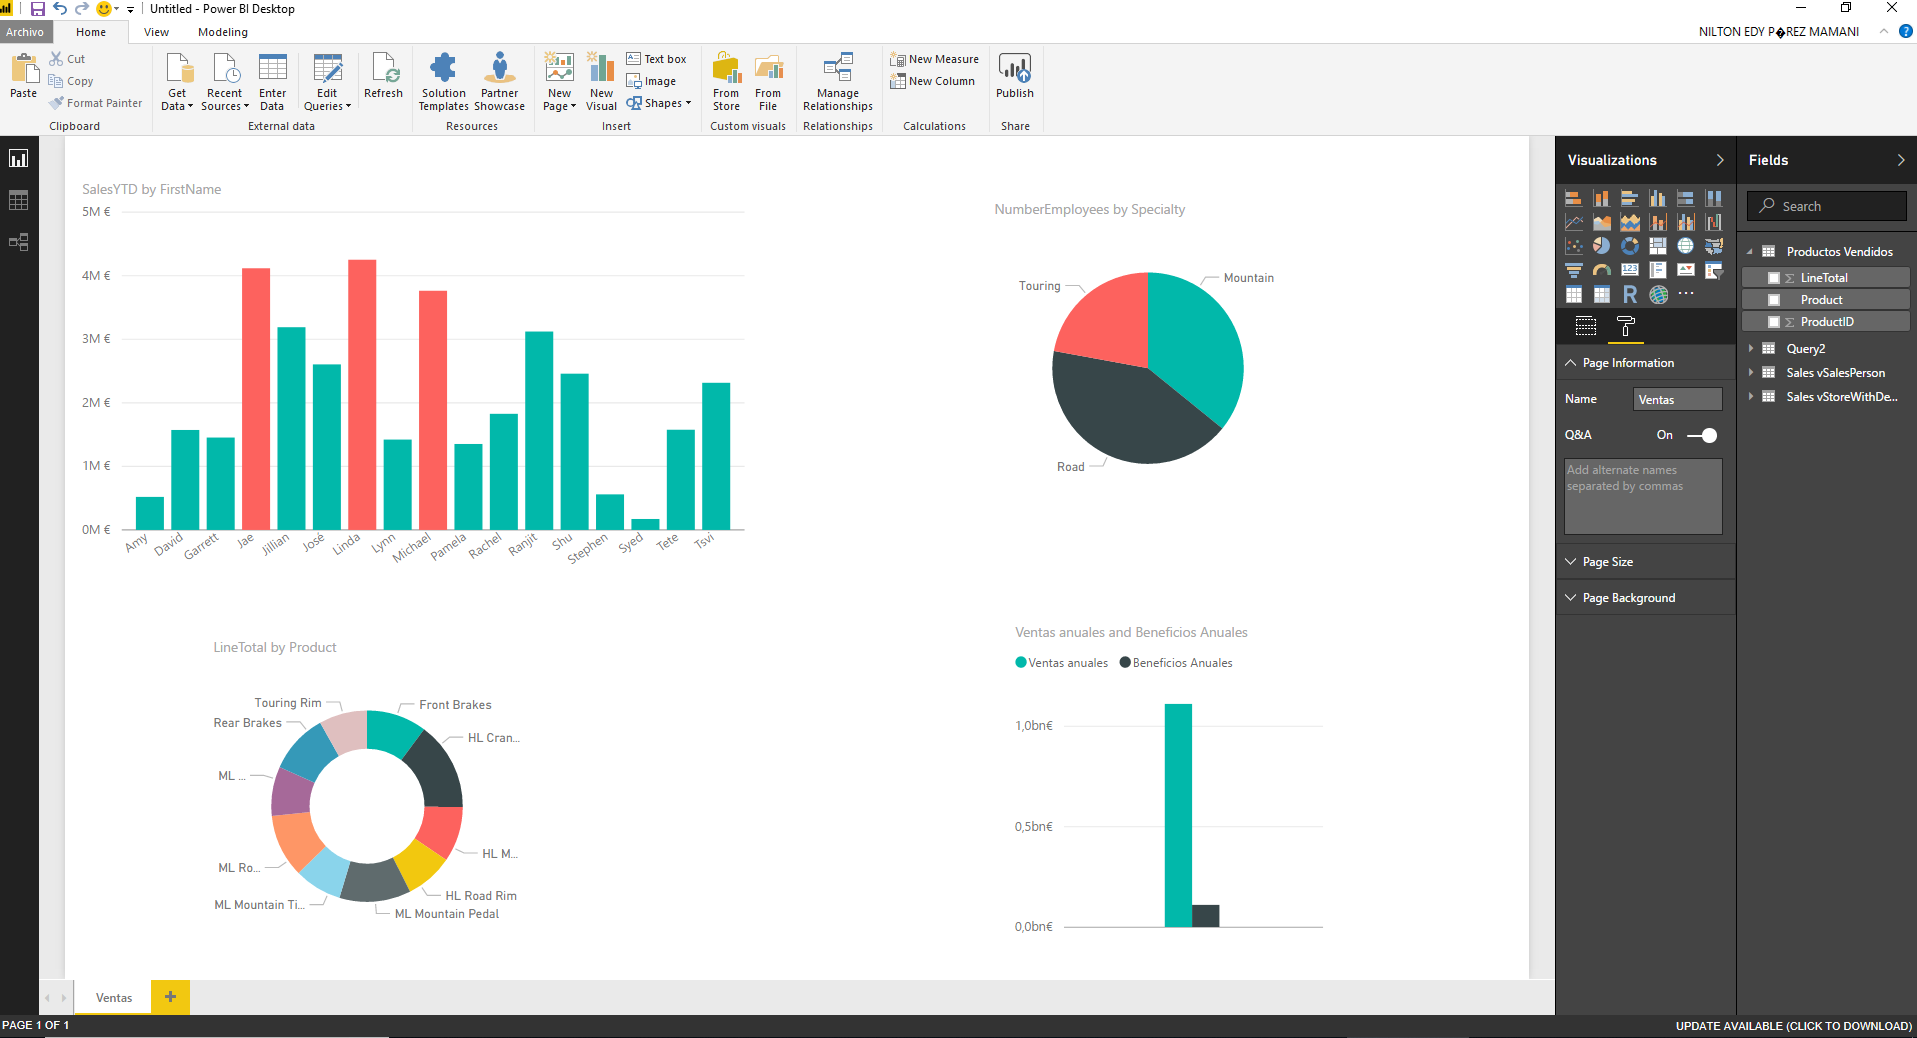
\includegraphics[width=15cm]{./Imagenes/imagen4} 
\end{center}

\begin{itemize}
5. Publicar el reporte en el portal de Power BI
\end{itemize}

\begin{center}
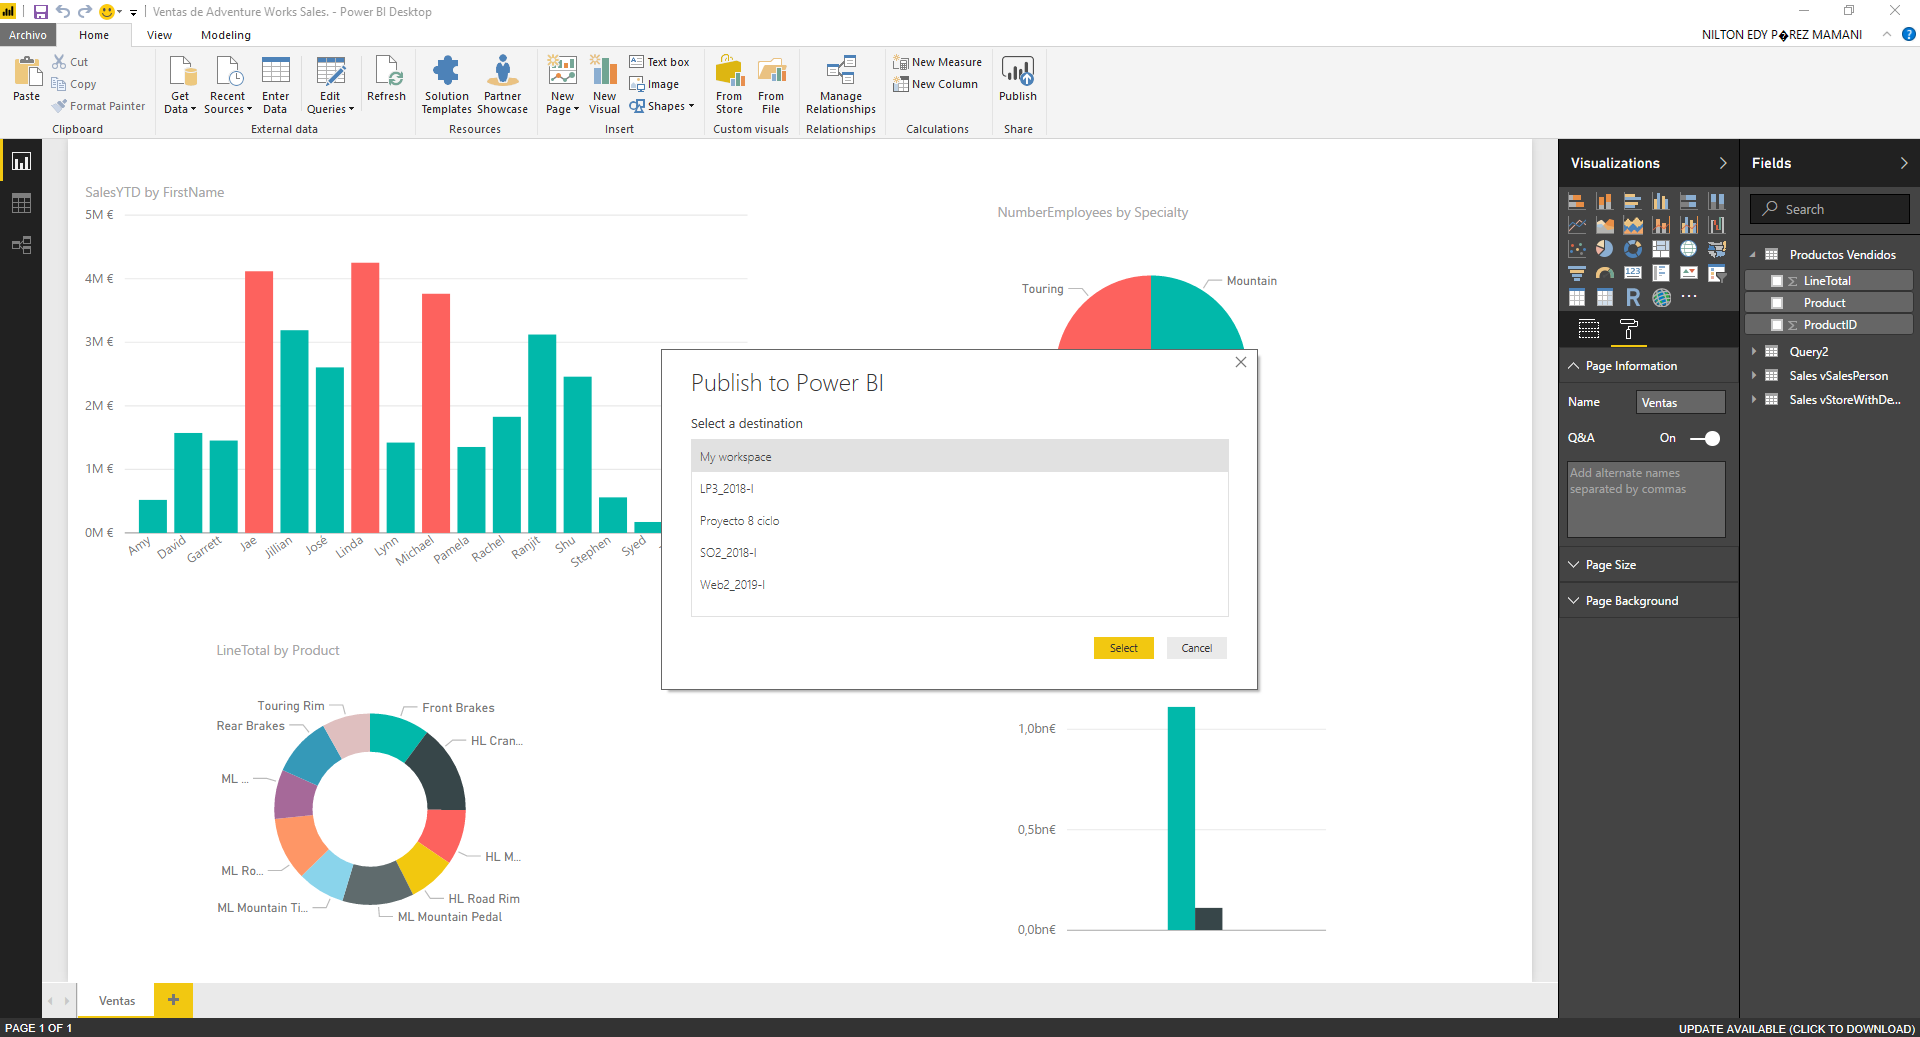
\includegraphics[width=15cm]{./Imagenes/imagen5} 
\end{center}

\begin{itemize}
6. Resultado final
\end{itemize}

\begin{center}
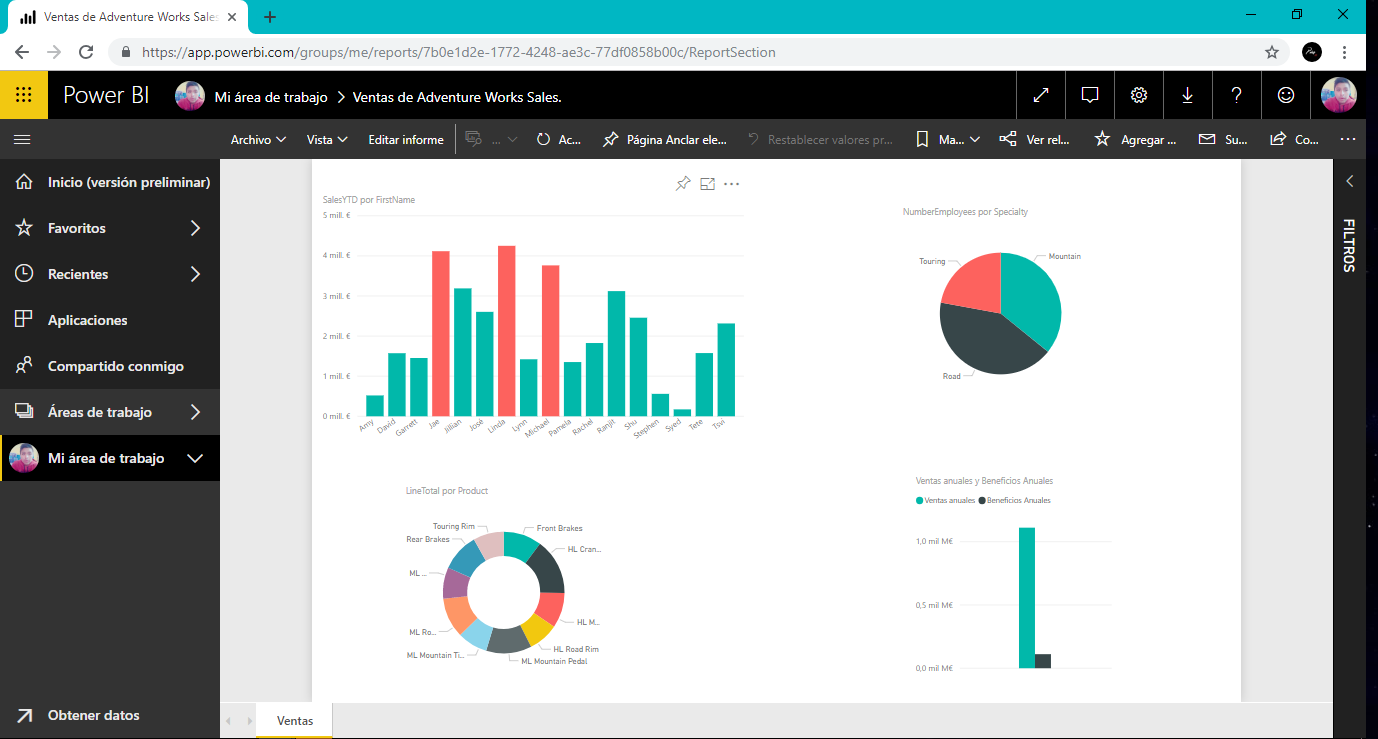
\includegraphics[width=15cm]{./Imagenes/imagen6} 
\end{center}